\begin{name}
	{\tenchude}
	{TOÁN 10}
	{LỚP TOÁN THẦY PHÁT}
	{{Không biết thì không có gì xấu hổ.\\ Chỉ nên cảm thấy xấu hổ khi không chịu học hỏi.}}
\end{name}
\Opensolutionfile{ansbook}[ans/ansbookDe7]
\TN
\Opensolutionfile{ans}[ans/ansDe1-TN7]
\begin{ex}%[Mức 2]%[H]giảng 10 New - 4in1, Nguyễn Vân Trường]%[0D3H1-5]
Cho hàm số $y=2 x^2-4x+3$. Mệnh đề nào sau đây \textbf{sai}?
\choice
{Hàm số đồng biến trong khoảng $(1;+\infty)$}
{Hàm số nghịch biến trong khoảng $(-\infty;1)$}
{Hàm số nghịch biến trong khoảng $(-\infty;-1)$}
{\True Hàm số đồng biến trong khoảng $(-1;+\infty)$}
\loigiai{
Hàm số bậc hai có $a=2>0$ và $-\dfrac{b}{2a}=1$ nên có bảng biến thiên:
\begin{center}

\begin{tikzpicture}[scale=1.2,>=stealth]
\tkzTabInit[nocadre=false,lgt=1,espcl=2,deltacl=0.5]{$x$/.7,$y$/2}
{$-\infty$ , $1$ , $+\infty$}
\tkzTabVar{+/$+\infty$ , -/$1$ , +/$+\infty$}
\end{tikzpicture}
\end{center}
Mệnh đề sai là: \lq\lq Hàm số cũng nghịch biến trên khoảng $(-\infty;-1)$ và không đồng biến trên khoảng $(-1;+\infty)$\rq\rq.
}
\end{ex}

\begin{ex}%[10-11-EX-GHK2-24-25]%[Dự Đỗ]%[0D3N2-1]
Trục đối xứng của đồ thị hàm số $y=a x^2+b x+c,(a \neq 0)$ là đường thẳng nào dưới đây?
\choice
{$x=-\dfrac{\Delta}{4a}$}
{$x=-\dfrac{c}{a}$}
{$y=-\dfrac{b}{2a}$}
{\True$x=-\dfrac{b}{2a}$}
\loigiai{
Trục đối xứng của đồ thị hàm số $y=a x^2+b x+c,(a \neq 0)$ là đường thẳng $x=-\dfrac{b}{2a}$.
}
\end{ex}

\begin{ex}%[0D3H2-2]
Hàm số nào sau đây có bảng biến thiên như hình dưới?
\begin{center}
\begin{tikzpicture}
\draw[thick](-6,4)--(-6,0) (-7,2.8)--(3,2.8);
\path (-6.5,3.45)node{$x$} (-5.5,3.45)node[]{$-\infty$} (2.5,3.35)node[]{$+\infty$} (-1.45,3.45)node[]{$1$} (-6.55,1)node[]{$y$} (-5.5,0.4)node[]{$-\infty$} (-1.5,2)node[]{$2$} (2.6,0.4)node[]{$-\infty$};
\draw[->] (-5.15,0.44)--(-2.03,2.12); \draw[->](-1.02,2.12)--(2.14,0.44);
\end{tikzpicture}
\end{center}
\choice
{$y=-x^2+5x+2$}
{\True $y=-\dfrac{1}{2}x^2+x$}
{$y=x^2-3x+1$}
{$y=\dfrac{1}{4}x^2-x+3$}
\loigiai{Dựa vào bảng biến thiên, hàm số cần tìm có $a<0$ và $\dfrac{b}{2a}=\dfrac{1}{2}$. Vậy chỉ có $y=-\dfrac{1}{2}x^2+x$ thỏa điều kiện trên.
}
\end{ex}

\begin{ex}%[H]%[Nguyễn Văn Cường (Cường NV) - Dự án giảng K10 - K11]%[0D6H1-1]
Cho giá trị gần đúng của $\dfrac{23}{7}$ là $3{,}28$. Sai số tuyệt đối của số $3{,}28$ là
\choice
{$0{,}04$}
{\True $\dfrac{0,04}{7}$}
{$0{,}06$}
{Đáp án khác}
\loigiai{
Ta có $\dfrac{23}{7} = 3{,}(285714) \Rightarrow\left|\dfrac{23}{7} - 3{,}28\right| = 0{,}00(571428) = \dfrac{0{,}04}{7}$.}
\end{ex}

\begin{ex}%[0-HK1-CTST-2-NguyenDu-2324]%[VN-MT-6, Lê Minh Thiện Anh]%[0D6H4-2]
Thu thập thông tin về thời gian (giờ) tham gia hoạt động ngoại khóa trong một tháng của học sinh của lớp 10A được cho bởi bảng sau:
\begin{center}
\begin{tabular}{|c|c|c|c|c|c|}
\hline Thời gian (giờ) & $2$ & $3$ & $4$ & $5$ & $6$ \\
\hline Số học sinh lớp 10A & $7$ & $9$ & $10$ & $8$ & $15$ \\
\hline
\end{tabular}
\end{center}
Khoảng biến thiên của lớp 10A là
\choice
{$1$}
{\True $4$}
{$22$}
{$8$}
\loigiai{
Khoảng biến thiên của lớp $10A$ là $R=6-2=4$.
}
\end{ex}

\begin{ex}%[0D0N1-2]%[Dự án đề kiểm tra Toán khối 10 HKI NH23-24-Dot 15- Hồ Văn Trung]%[THPT Lê Qúy Đôn- TPHCM]
Bạn Minh muốn nuôi một trong bốn con vật sau: mèo, chó, chim, cá. Bạn Minh đã chọn ngẫu nhiên một con vật. Tập hợp nào sau đây \textbf{không phải} là một biến cố của phép thử trên?
\choice
{$H=\varnothing $}
{$K= \{ \text{mèo, chó, chim, cá}\}$}
{\True $J= \{ \text{mèo, chim, thỏ}\}$}
{$I= \{ \text{chó, cá}\}$}
\loigiai{Ta có thỏ không phải là con vật bạn Minh nuôi.\\
Nên tập $J= \{ \text{mèo, chim, thỏ}\}$ không phải là một biến cố của phép thử trên.
}
\end{ex}

\begin{ex}%[0D0N1-3]
Một cửa hàng có $23$ chiếc kem que khác nhau và $7$ chiếc kem ốc quế khác nhau. Chọn ngẫu nhiên một chiếc kem que và một chiếc kem ốc quế. Số phần tử của không gian mẫu là
\choice
{\True $161$}
{$30$}
{$35$}
{$435$}
\loigiai{
Số phần tử của không gian mẫu là $n(\Omega)=23\cdot7=161$.
}
\end{ex}

\begin{ex}%[10-11-EX-GHK2-2425]%[Lê Toàn]%[0H9H3-1]
Cho đường thẳng $d \colon \heva{&x=5+t \\&y=-9-2t}$; khẳng định nào sau đây \textbf{sai}?
\choice
{$d$ có véc-tơ chỉ phương $(1;-2)$}
{$d$ có véc-tơ pháp tuyến $(2;1)$}
{$d$ có véc-tơ chỉ phương $(2;-4)$}
{\True $d$ có véc-tơ pháp tuyến $(2;-1)$}
\loigiai{
Đường thẳng $d$ có véc-tơ chỉ phương $\overrightarrow{u}=(1;-2)$  nên có một véc-tơ pháp tuyến là $\overrightarrow{n}=(2;1)$.
}
\end{ex}

\begin{ex}%[0H9H3-2]%[Dự án đề kiểm tra Toán 11 GHKII NH23-24-Nguyen Tran Anh Tuan]%[THPT Thiệu Hóa - Thanh Hóa]
Trong mặt phẳng tọa độ $Oxy$ đường thẳng đi qua $A(-1; 4)$ và song song trục $Ox$ có phương trình là
\choice
{$x-1=0$}
{$y+4=0$}
{$x+1=0$}
{\True $y-4=0$}
\loigiai{
Gọi $d$ là đường thẳng cần tìm.\\
Vì $d \parallel Ox \Rightarrow \overrightarrow{u_d}=\overrightarrow{u}_{Ox}=(1; 0)$ suy ra $\overrightarrow{n_d}=(0;-1)$.\\
Phương trình tổng quát của $d$ là $(d)\colon 0(x+1)-1(y-4)=0$ hay $ y-4=0$.
}
\end{ex}

\begin{ex}%[0H9H3-4]%[Tex hóa đề CK2 - form 2025 - đọt 2 -Huỳnh Thanh Chí]
Cho 2 đường thẳng $\Delta\colon x-y+2=0$ và $\Delta'\colon-x+1=0$. Góc giữa 2 đường thẳng $\Delta$ và $\Delta'$ bằng
\choice
{$90^{\circ}$}
{$135^{\circ}$}
{\True $45^\circ$}
{$60^{\circ}$}
\loigiai{Ta có véc-tơ pháp tuyến của $\Delta$ là $\overrightarrow{n}=(1;-1)$, véc-tơ pháp tuyến $\Delta'$ là $\overrightarrow{n}'=(1; 0)$.\\
Ta có $
\cos \left(\Delta, \Delta'\right)=\left|\cos \left(\overrightarrow{n}, \overrightarrow{n}'\right)\right|=\dfrac{\sqrt{2}}{2} \Rightarrow\left(\Delta, \Delta'\right)=45^{\circ}$.
}
\end{ex}

\begin{ex}%[0H9N5-1]
Trong mặt phẳng $O x y$, tọa độ các tiêu điểm của elip có phương trình chính tắc \break $\dfrac{x^2}{25}+\dfrac{y^2}{16}=1$ là
\choice
{\True $F_1(-3 ; 0)$; $F_2(3 ; 0)$}
{$F_1(0 ;-4)$; $F_2(0 ; 4)$}
{$F_1(-4 ; 0)$; $F_2(4 ; 0)$}
{$F_1(0 ;-3)$; $F_2(0 ; 3)$}
\loigiai{ Ta có $\heva{&a^2=25\\&b^2=16}\Rightarrow c^2=a^2-b^2=25-16=9.$\\
Tọa độ các tiêu điểm của elip là $F_1(-3 ; 0)$; $F_2(3 ; 0)$.
}
\end{ex}

\begin{ex}%[0H9N5-5]%[Dự án đề kiểm tra Toán 10 HKII NH23-24- Đoàn Minh Tâm]%[THPT Mạc Đĩnh Chi]
Trong mặt phẳng tọa độ $Oxy$, hypebol $(H)$ có độ dài trục thực bằng $ 6$ và tiêu cự bằng $ 10$ có phương trình chính tắc là
\choice
{\True $(H)\colon\dfrac{x^2}{9}-\dfrac{y^2}{16}=1$}
{$(H)\colon\dfrac{x^2}{16}-\dfrac{y^2}{9}=1$}
{$(H)\colon\dfrac{x^2}{25}-\dfrac{y^2}{9}=1$}
{$(H)\colon\dfrac{x^2}{36}-\dfrac{y^2}{64}=1$}
\loigiai{
Độ dài trục thực bằng $6$ nên $2a=6 \Rightarrow a=3\Rightarrow a^2=9$.\\
Tiêu cự bằng $10$ nên $2c=10 \Rightarrow c=5$.\\
Ta có $b^2=c^2-a^2=25-9=16$.\\
Vậy phương trình chính tắc của hypebol $(H)$ là $\dfrac{x^2}{9}-\dfrac{y^2}{16}=1$.
}
\end{ex}
\TNTF
\begin{ex}%[0D6H4-2]
Số áo bán được trong một tháng ở cửa hàng bán áo sơ mi nam được thống kê như sau:
\begin{center}
\begin{tabular}{|c|c|c|c|c|c|c|c|c|}
\hline
Cỡ áo&36&37&38&39&40&41&42&Tổng\\
\hline
Tần số (Số áo bán được) &3&11&32&31&27&10&65&179\\
\hline
\end{tabular}
\end{center}
Các mệnh đề sau đúng hay \textbf{sai}?
\choiceTF
{Mốt của mẫu số liệu là $65$}
{\True Số trung bình của mẫu số liệu là $40$}
{Khoảng biến thiên của mẫu số liệu là $62$}
{\True Trung vị của mẫu số liệu là $40$}
\loigiai{
\begin{itemchoice}
\itemch Cỡ áo bán được nhiều nhất là $42$. Suy ra Mốt của mẫu số liệu là $42$ nên mệnh đề sai.
\itemch Số trung bình của mẫu số liệu là
\[\overline{x}=\dfrac{1}{179}\left(36\cdot3+37\cdot11+38\cdot32+39\cdot31+40\cdot27+41\cdot10+42\cdot65\right)=40\]
nên mệnh đề đúng.
\itemch Khoảng biến thiên của mẫu số liệu là: $R=42-36=6$ nên mệnh đề sai.
\itemch Vì số giá trị của mẫu số liệu là 179 (số lẻ) nên trung vị là số chính giữa, $Me=x_{90}=40$. Do đó mệnh đề đúng.
\end{itemchoice}
}
\end{ex}

\begin{ex}%[0H9H3-2]%[Làm đề GHK, HK, 4 phần - 2025]%[Huỳnh Xuân Tín]
Trong mặt phẳng toạ độ $Oxy$, cho tam giác $ABC$ có $A(3; 4)$, đường trung trực cạnh $BC$ có phương trình $3x-y+1=0$, đường trung tuyến kẻ từ $C$ có phương trình $2x-y+5=0$. Xét tính đúng sai các mệnh đề sau
\choiceTF
{Gọi $M$ là trung điểm cạnh $BC$. Khi đó $M(9; 39)$}
{Phương trình đường thẳng $BC$ là $x+3y-63=0$}
{Tọa độ đỉnh $C$ là $C(-1; 3)$}
{Tọa độ đỉnh $B$ là $B\left(\dfrac{15}{7}; \dfrac{142}{7}\right)$}
\loigiai{
\begin{itemchoice}
\itemch Sai. Gọi $M$ là trung điểm cạnh $BC$. Vì $M$ nằm trên đường trung trực cạnh $BC$ nên giả sử $M\ (t; 3t+1)$.\\
Gọi $G$ là trọng tâm tam giác $ABC$. Vì $G$ nằm trên đường trung tuyến kẻ từ $C$ nên giả sử $G\ (s; 2s+5)$.\\
Ta có $\heva{& \overrightarrow{A M}=(t-3; 3 t-3)\\&\overrightarrow{A G}=(s-3; 2 s+1).}$\\
Khi đó
\begin{eqnarray*}
& &\overrightarrow{A M}=\dfrac{3}{2} \overrightarrow{A G}\\ &\Leftrightarrow&\heva{&t-3=\dfrac{3}{2}(s-3)\\&3t-3=\dfrac{3}{2}(2s+1)}\\
&\Leftrightarrow& \heva{&{2t-3s=-3} \\&{6t-6s=9}}\\
&\Leftrightarrow& \heva{&t=\dfrac{15}{2} \\	&s=6.}
\end{eqnarray*}
Suy ra $M\left(\dfrac{15}{2}; \dfrac{47}{2}\right)$.
\itemch Sai. Đường thẳng $BC$ đi qua $M\left(\dfrac{15}{2}; \dfrac{47}{2}\right)$ và vuông góc với đường thẳng $3x-y+1=0$ nên ta có phương trình đường thẳng $BC$ là\\ $1\cdot\left(x-\dfrac{15}{2}\right)+3\cdot\left(y-\dfrac{47}{2}\right)=0\Leftrightarrow x+3y-78=0$.
\itemch Sai. Toạ độ đỉnh $C$ là nghiệm của hệ phương trình $\heva{&x+3y-78=0\\
&2x-y+5=0} \Leftrightarrow\heva{&x=9 \\&y=23.}$
\itemch Sai. Ta có $C\left(9; 23\right)$.Vì $M$ là trung điểm $BC$ nên $B\left(6; 24\right)$.
\end{itemchoice}}
\end{ex}
\TNSA
\begin{ex}%[Dự án Form mới 12/4/6-HK1 Lớp 10-11]%[VN-MT-6, Võ NGuyên Thạch]%[THPT TÂN TÚC-TP HCM]%[0D3H2-3]
Biết hàm số $y=x^2-2x-1$ nghịch biến trên khoảng $(-\infty;a)$ và đồng biến trên khoảng $(a;+\infty)$. Tìm $a$.
\shortans{$1$}
\loigiai{
\begin{itemize}
\begin{multicols}{2}
\item Hàm số $y=x^2-2x-1$.
\item Tập xác định: $\mathscr{D}=\mathbb{R}$.
\item Trục đối xứng: $x=1$.
\item Đỉnh $S(1;-2)$.
\end{multicols}
\item Bảng biến thiên.
\begin{center}
\begin{tikzpicture}[font=\normalsize,t style/.style={style=solid}]
%dòng khai báo
\tkzTabInit[nocadre=true,lgt=1,espcl=4,deltacl=0.5]
{$x$ /0.7, $y$/2}
{$ -\infty$,$1$,$+\infty$}
%dòng biến thiên
\path ($(N11)!0.2!(N12)$) node (A1){$+\infty$}
($(N21)!0.9!(N22)$) node (A2){$ -2 $}
($(N31)!0.2!(N32)$) node (A3){$ +\infty $};
\foreach \x/\y in {A1/A2,A2/A3}{
\draw[-stealth] (\x)--(\y);
}
\end{tikzpicture}
\end{center}
\item Nhận xét: Hàm số đồng biến trên $(1;+\infty)$, hàm số nghịch biến trên $(-\infty;1)$.
\end{itemize}
Vậy $a=1$.
}
\end{ex}

\begin{ex}%[0D7V2-7]
Một cửa hàng buôn giày nhập một đôi giày với giá $40$ nghìn đồng. Cửa hàng ước tính rằng nếu đôi giày được bán với giá $x$ nghìn đồng thì mỗi tháng khách hàng sẽ mua $(120-x)$ đôi. Hỏi cửa hàng bán một đôi giày với giá tối đa bao nhiêu nghìn đồng thì tháng đó cửa hàng có lợi nhuận không thấp hơn $1\,200\,000$ đồng?
\shortans{$100$}
\loigiai{
Số tiền lãi của cửa hàng trong một tháng là
\[
f(x)=(120-x)(x-40)=-x^2+160 x-4800~\text{(nghìn đồng)}.
\]
Để cửa hàng có lợi nhuận không thấp hơn $1\,200$ nghìn đồng trong tháng đó thì
\[
f(x)\geq 1200 \Leftrightarrow-x^2+160 x-4800\geq 1200 \Leftrightarrow 60\leq x\leq 100.
\]
Vậy cửa hàng có thể bán một đôi giày với giá tối đa $100$ nghìn đồng.
}
\end{ex}

\begin{ex}%[0-HK1-CT-4-THTHDHSG-HCM-2324]%[VN-MT-6, VM026]%[0D6H3-2]
Thống kê độ tuổi kiếm được việc làm đúng chuyên ngành sau khi tốt nghiệp đại học của một nhóm người, thu được bảng sau
\begin{center}
\begin{tabular}{|c|c|c|c|c|c|}
\hline
Tuổi		& 22& 23& 24& 25& 26 \\
\hline
Số người 	& 12& 20& 19& 8& 5\\
\hline
\end{tabular}
\end{center}
Tính độ tuổi trung bình của nhóm người này khi họ kiếm được việc làm đúng chuyên ngành (kết quả làm tròn đến chữ số hàng phần mười).
\shortans{$23{,}6$}
\loigiai{
Ta có, cỡ mẫu $n=12+20+19+8+5=64$.\\
Độ tuổi trung bình của nhóm người này khi họ kiếm được việc làm đúng chuyên ngành được tính là
\[\overline{x}=\dfrac{12\cdot 22 + 20 \cdot 23 + 19 \cdot 24 + 8 \cdot 25+5 \cdot 26}{64}=\dfrac{1510}{64}\approx23{,}6.\]
}
\end{ex}

\begin{ex}%[0H9V4-2]
Trong mặt phẳng với hệ tọa độ $Oxy$, cho đường thẳng $d\colon 2x-y-5=0$ và hai điểm $A\left(1;2\right), B\left(4;1\right)$. Tính bán kính đường tròn $(C)$ có tâm thuộc $d$ và đi qua hai điểm $A, B$.
\shortans{$5$}
\loigiai{
\immini{
Gọi $I$ là tâm của $(C)$. Do $I\in d$ nên $I\left(t;2t-5\right)$.\\
Hai điểm $A, B$ cùng thuộc $(C)$ nên
\begin{align*}
IA=IB & \Leftrightarrow (1-t)^2+\left(7-2t\right)^2=(4-t)^2+\left(6-2t\right)^2\\
& \Leftrightarrow t=1.
\end{align*}
Suy ra $I(1;-3)$ và bán kính $R=IA=5$.\\

}
{
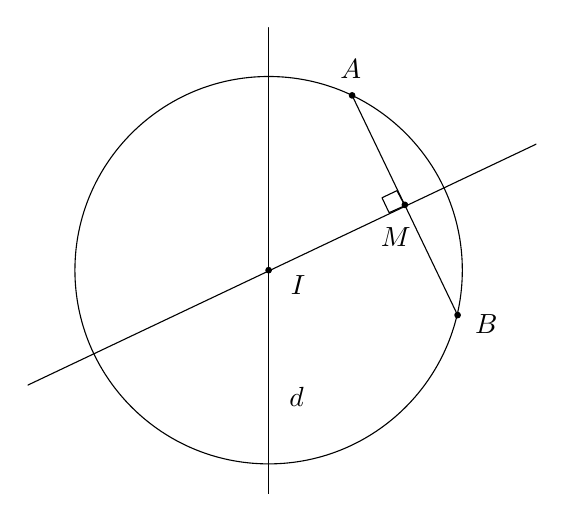
\begin{tikzpicture}[line cap=round,line join=round,>=stealth,x=1.0cm,y=1.0cm]
\clip(1.24,-1.) rectangle (7.7,4.92);
\draw (5.93,2.85) -- (5.74,2.76) -- (5.83,2.57) -- (6.03,2.66) -- cycle;
\draw (4.3,1.84) circle (2.46cm);
\draw (5.36,4.06)-- (6.7,1.27);
\draw [domain=1.24:7.7] plot(\x,{(-0.36--0.82*\x)/1.73});
\draw (4.3,-1.) -- (4.3,4.92);
\draw (5.6,4.4) node[left] {$A$};
\draw (6.8,1.4) node[anchor=north west] {$B$};
\draw (5.6,2.5) node[anchor=north west] {$M$};
\draw (4.44,0.48) node[anchor=north west] {$d$};
\draw (4.46,1.9) node[anchor=north west] {$I$};
\draw [fill=black] (4.3,1.84) circle (1.0pt);
\draw [fill=black] (5.36,4.06) circle (1.0pt);
\draw [fill=black] (6.7,1.27) circle (1.0pt);
\draw [fill=black] (6.03,2.67) circle (1.0pt);
\end{tikzpicture}
}
}
\end{ex}
\TL
\begin{ex}%[Kiểm tra cuối kỳ 1- Trường THPT Nguyễn Thượng Hiền, Tp HCM, 2023-2024]%[Phạm Phương - 10-11EX-HK1]%[0D3H1-2]
%Câu 3: (1,0 điểm)
Tìm tập xác định của hàm số $f(x)=\dfrac{x-1}{x^2-3x+2}+\sqrt{4-2x}$.
\loigiai{
Hàm số $f(x)=\dfrac{x-1}{x^2-3x+2}+\sqrt{4-2x}$ xác định khi
$\heva{&x^2-3x+2\neq 0 \\& 4-2x\geq 0}
\Leftrightarrow \heva{&x\neq 1\\&x\neq 2\\&x\leq 2.}$\\
Vậy tập xác định của hàm số đã cho là $\mathscr{D}=\left(-\infty;2\right]\setminus\left\{1;2\right\}=\left(-\infty;2\right)\setminus\left\{1\right\}$.
}
\end{ex}

\begin{ex}%[0D7V3-6]
Một người đi bộ xuất phát từ $B$ trên một bờ sông (coi là đường thẳng) với vận tốc $6$ km/h để gặp một người chèo thuyền xuất phát cùng lúc từ vị trí $A$ với vận tốc $3$ km/h. Nếu người chèo thuyền di chuyển theo đường vuông góc với bờ thì phải đi một khoảng cách $A H=300$ m và gặp người đi bộ tại địa điểm cách $B$ một khoảng $B H=1\,400$ m. Tuy nhiên, nếu di chuyển theo cách đó thì hai người không tới cùng lúc. Để hai người đến cùng lúc thì mỗi người cùng di chuyển về vị trí $C$ (Hình dưới).  Tính số phút từ khi hai người xuất phát cho đến khi gặp nhau.
\begin{center}
\begin{tikzpicture}[scale=.8, >=stealth]
\coordinate [label=  below left:$H$](H) at (0,0);
\coordinate [label=below right:$B$](B) at (9.25,0);
\coordinate [label=above:$A$](A) at (0,5);
\coordinate [label=below:$C$](C) at (2.54,0);
\foreach \diem in {H,B,A,C}	\fill (\diem)circle(1.5pt);
\draw[smooth](-1,0)--(11,0) (H)--(A)--(C) (A)--(B);
\draw ($(H)!.5!(A)$) node[left]{$300$ m};
\draw ($(B)!.5!(A)$) node[above right]{$200$ m};
\draw[dashed](B)--($(B)-(0,1.5)$) (H)--($(H)-(0,1.5)$);
\draw[<->,dashed]($(B)-(0,1)$)--($(H)-(0,1)$);
\draw (4.5,-1) node[below]{$1\,400$ m};
\end{tikzpicture}
\end{center}
\loigiai{Đặt $C H=x$ (m) $(x>0)$. Ta có $A C=\sqrt{300^2+x^2}$, $C B=1400-x$.\\
Vì hai người gặp nhau cùng lúc tại $C$ nên \[\dfrac{\sqrt{300^2+x^2}}{3\,000}=\dfrac{1\,400-x}{6\,000} \Leftrightarrow 2 \sqrt{300^2+x^2}=1\,400-x.\]
Giải phương trình trên ta có $x=400$ (m) với $x>0$. Suy ra $CB=1\,400-400=1\,000$ (m).\\Thời gian hai người bắt đầu di chuyển cho đến khi tới $C$ là $10$ phút.
}
\end{ex}

\begin{ex}%[Phan Quốc Trí]%[0D0C2-7]
Gọi $X$ là tập hợp các số tự nhiên chẵn có $4$ chữ số khác nhau được lập từ các chữ	số $0$; $2$; $3$; $4$; $5$; $6$; $7$. Chọn ngẫu nhiên một số thuộc tập $X$. Tính xác suất để số được chọn chia hết cho $4$ (làm tròn đến hàng phần nghìn).
% \shortans{$0{,}495$}
\loigiai
{
Gọi $\overline{abcd}$ là số tự nhiên chẵn có $4$ chữ số khác nhau được lập từ các chữ số $0$; $2$; $3$; $4$; $5$; $6$; $7$.\\ Các khả năng xảy ra là
\begin{itemize}
\item $d=0$: $a$ có $6$ cách chọn, $b$ có $5$ cách chọn, $c$ có $4$ cách chọn. Có $6\cdot 5\cdot 4=120$ số như vậy.
\item $d\in \{2;4;6\}\Rightarrow d$ có $3$ cách chọn, $a$ có $5$ cách chọn, $b$ có $5$ cách chọn, $c$ có $4$ cách chọn. Có $3\cdot 5\cdot 5\cdot 4=300$ số như vậy.
\end{itemize}
Số phần tử của không gian mẫu là $n(\Omega)=120+300=420$.\\
Gọi $A$ là biến cố \lq\lq Số được chọn chia hết cho $4$\rq\rq.\\
Các khả năng xảy ra là
\begin{itemize}
\item $\overline{cd}\in \{04;20;40;60\}$, $\overline{cd}$ có $4$ cách chọn, $a$ có $5$ cách chọn, $b$ có $4$ cách chọn. Có $4\cdot 5\cdot 4=80$ số như vậy.
\item $\overline{cd}\in \{24;32;36;52;56;64;72;76\}$, $\overline{cd}$ có $8$ cách chọn, $a$ có $4$ cách chọn, $b$ có $4$ cách chọn.\\ Có $8\cdot 4\cdot 4=128$ số như vậy.
\end{itemize}
Số phần tử của biến cố $A$ là $n(A)=80+128=208$.\\
Xác suất cần tìm là $\mathrm{P}(A)=\dfrac{n(A)}{n(\Omega)}=\dfrac{208}{420}=\dfrac{52}{105} \approx 0{,}495$.
}
\end{ex}
\Closesolutionfile{ans}
\Closesolutionfile{ansbook}
